%%%%%%%%%%%%%%%%%%%%%%%%%%%%%%%%%%%%%%%%%
% Beamer Presentation
% LaTeX Template
% Version 1.0 (10/11/12)
%
% This template has been downloaded from:
% http://www.LaTeXTemplates.com
%
% License:
% CC BY-NC-SA 3.0 (http://creativecommons.org/licenses/by-nc-sa/3.0/)
%
%%%%%%%%%%%%%%%%%%%%%%%%%%%%%%%%%%%%%%%%%

%----------------------------------------------------------------------------------------
%	PACKAGES AND THEMES
%----------------------------------------------------------------------------------------

\documentclass{beamer}

\mode<presentation> {

% The Beamer class comes with a number of default slide themes
% which change the colors and layouts of slides. Below this is a list
% of all the themes, uncomment each in turn to see what they look like.

%\usetheme{default}
%\usetheme{AnnArbor}
%\usetheme{Antibes}
%\usetheme{Bergen}
%\usetheme{Berkeley}
%\usetheme{Berlin}
%\usetheme{Boadilla}
%\usetheme{CambridgeUS}
%\usetheme{Copenhagen}
%\usetheme{Darmstadt}
%\usetheme{Dresden}
%\usetheme{Frankfurt}
%\usetheme{Goettingen}
%\usetheme{Hannover}
%\usetheme{Ilmenau}
%\usetheme{JuanLesPins}
%\usetheme{Luebeck}
\usetheme{Madrid}
%\usetheme{Malmoe}
%\usetheme{Marburg}
%\usetheme{Montpellier}
%\usetheme{PaloAlto}
%\usetheme{Pittsburgh}
%\usetheme{Rochester}
%\usetheme{Singapore}
%\usetheme{Szeged}
%\usetheme{Warsaw}

% As well as themes, the Beamer class has a number of color themes
% for any slide theme. Uncomment each of these in turn to see how it
% changes the colors of your current slide theme.

%\usecolortheme{albatross}
%\usecolortheme{beaver}
%\usecolortheme{beetle}
%\usecolortheme{crane}
%\usecolortheme{dolphin}
%\usecolortheme{dove}
%\usecolortheme{fly}
%\usecolortheme{lily}
%\usecolortheme{orchid}
%\usecolortheme{rose}
%\usecolortheme{seagull}
%\usecolortheme{seahorse}
%\usecolortheme{whale}
%\usecolortheme{wolverine}

%\setbeamertemplate{footline} % To remove the footer line in all slides uncomment this line
%\setbeamertemplate{footline}[page number] % To replace the footer line in all slides with a simple slide count uncomment this line

%\setbeamertemplate{navigation symbols}{} % To remove the navigation symbols from the bottom of all slides uncomment this line
}

\usepackage{graphicx} % Allows including images
\usepackage{booktabs} % Allows the use of \toprule, \midrule and \bottomrule in tables
\usepackage{multirow}
\usepackage{adjustbox}
\usepackage{array}
\usepackage{tikz}
\usepackage{soul}
\usetikzlibrary{shapes.geometric, arrows, positioning, fit}
\usepackage[latin1]{inputenc}
\newcommand{\xmark}{\textcolor{red}{\text{\sffamily X}}}
\newcommand{\cmark}{\textcolor{green}{\checkmark}}
\newcommand{\tr}{\text{tr}}
\newcommand{\E}{\textbf{E}}
\newcommand{\diag}{\text{diag}}
\newcommand{\argmax}{\text{argmax}}
\newcommand{\argmin}{\text{argmin}}
\newcommand{\Cov}{\text{Cov}}
\newcommand{\Var}{\text{Var}}
\newcommand{\Vol}{\text{Vol}}
\newcommand{\bx}{\boldsymbol{x}}
\newcommand{\by}{\boldsymbol{y}}
\newcommand{\bX}{\boldsymbol{X}}
\newcommand{\bY}{\boldsymbol{Y}}
\sethlcolor{gray}
\makeatletter
\newcommand\SoulColor{%
  \let\set@color\beamerorig@set@color
  \let\reset@color\beamerorig@reset@color}
\makeatother
\definecolor{color1}{RGB}{128,13,13}
\definecolor{color2}{RGB}{70,128,13}
\definecolor{color3}{RGB}{13,128,128}
\definecolor{color4}{RGB}{70,13,128}

%tikz stufff


%----------------------------------------------------------------------------------------
%	TITLE PAGE
%----------------------------------------------------------------------------------------


\title[Mutual information]{Estimating mutual information using sparse regression}

\author{Charles Zheng} % Your name
\institute[Stanford] % Your institution as it will appear on the bottom of every slide, may be shorthand to save space
{Stanford University}
\date{\today} % Date, can be changed to a custom date

\begin{document}

\begin{frame}
\titlepage % Print the title page as the first slide
(Joint work with Yuval Benjamini.)
\end{frame}


\section{Introduction}

\begin{frame}
\frametitle{Mutual information (Shannon 1948)}
\begin{center}
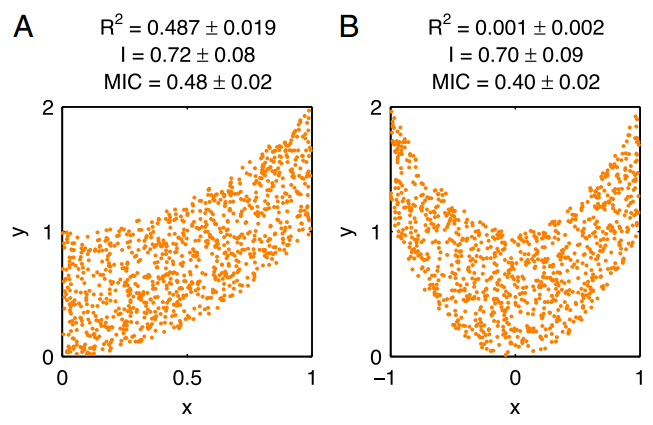
\includegraphics[scale = 0.2]{kinney.png}
\end{center}
\begin{itemize}
\item $I(X;Y) \in [0,\infty]$.  (0 if $X \perp Y$, $\infty$ if $X=Y$ and $X$ continuous.)
\item Symmetry: $I(X;Y) = I(Y; X)$.
\item Data-processing inequality
\[I(X; Y) \geq I(\phi(X); \psi(Y))\]
equality for $\phi$, $\psi$ bijections
%\item Additivity.  If $(X_1,Y_1) \perp (X_2, Y_2)$, then
%\[
%I((X_1, X_2); (Y_1, Y2)) = I(X_1; Y_1) + I(X_2; Y_2).
%\]
%\item Relation to KL divergence
%\[\mathbb{D}(p(x, y)||p(x)p(y)) = I(X; Y).\]
\end{itemize}
\tiny{Image credit Kinney et al. 2014.}
\end{frame}

\begin{frame}
\frametitle{Applications of $I(X; Y)$} 
\begin{itemize}
\item Feature selection (Peng et al. 2005, Fleuret 2004, Bennesar et al. 2015)
\item Structure learning for graphical models using conditional mutual information $I(X; Y|Z)$
(Vastano and Swinney 1988, Cheng et al. 1997, Bach and Jordan 2002)
\item Quantifying information capacity of neurons
\begin{center}
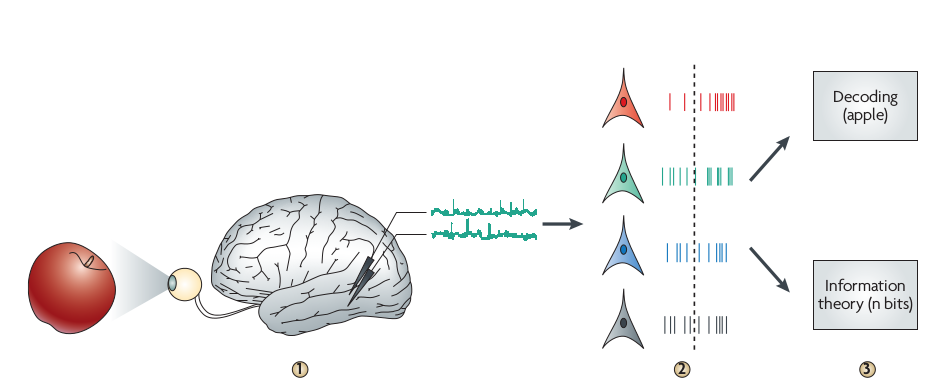
\includegraphics[scale = 0.2]{quiroga.png}
\end{center}
\tiny{Image credits: Quiroga et al. (2009).}
\end{itemize}
\end{frame}

\begin{frame}
\frametitle{How to estimate $I(X; Y)$}
Suppose we observe pairs $(X_i,Y_i)_{i=1}^n$ iid from density $p(x, y)$
\begin{itemize}
\item Definition of mutual information:
\[
I(X; Y) = \int \log \left(\frac{p(x, y)}{p(x)p(y)}\right) p(x, y) dx dy
\]
\item Simply using plugging in kernel density estimate $\hat{p}(x, y)$ leads to large bias (Beirlant et al. 2001)
\item Jackknifed estimate gives better result (Ivanov and Rozhkova 1981)
\[
\hat{I}(X; Y) = \frac{1}{n} \sum_{i=1}^n \log \left(\frac{\hat{p}_{-i}(x_i, y_i)}{\hat{p}_{-i}(x_i)\hat{p}_{-i}(y_i)}\right)
\]
\end{itemize}
\end{frame}

\begin{frame}
\frametitle{Problems in high dimensions}
\begin{itemize}
\item Density estimation is known to have exponential complexity with respect to dimensionality.
\item Many applications with high-dimensional $X$, $Y$.
\begin{itemize}
\item Gene expression time series
\item Functional magnetic resonance imaging
\end{itemize}
\item One approach is to assume joint multivariate normality of $X$, $Y$, but this reduces mutual information to a linear statistic.
\item Other approaches: binning (Bialek et al. 1991, Paninski 2003), confusion matrix of a classifier (Treves 1997, Quiroga et al. 2009).
\end{itemize}
\end{frame}


\begin{frame}
\frametitle{Idea: Use sparsity!}
\begin{center}
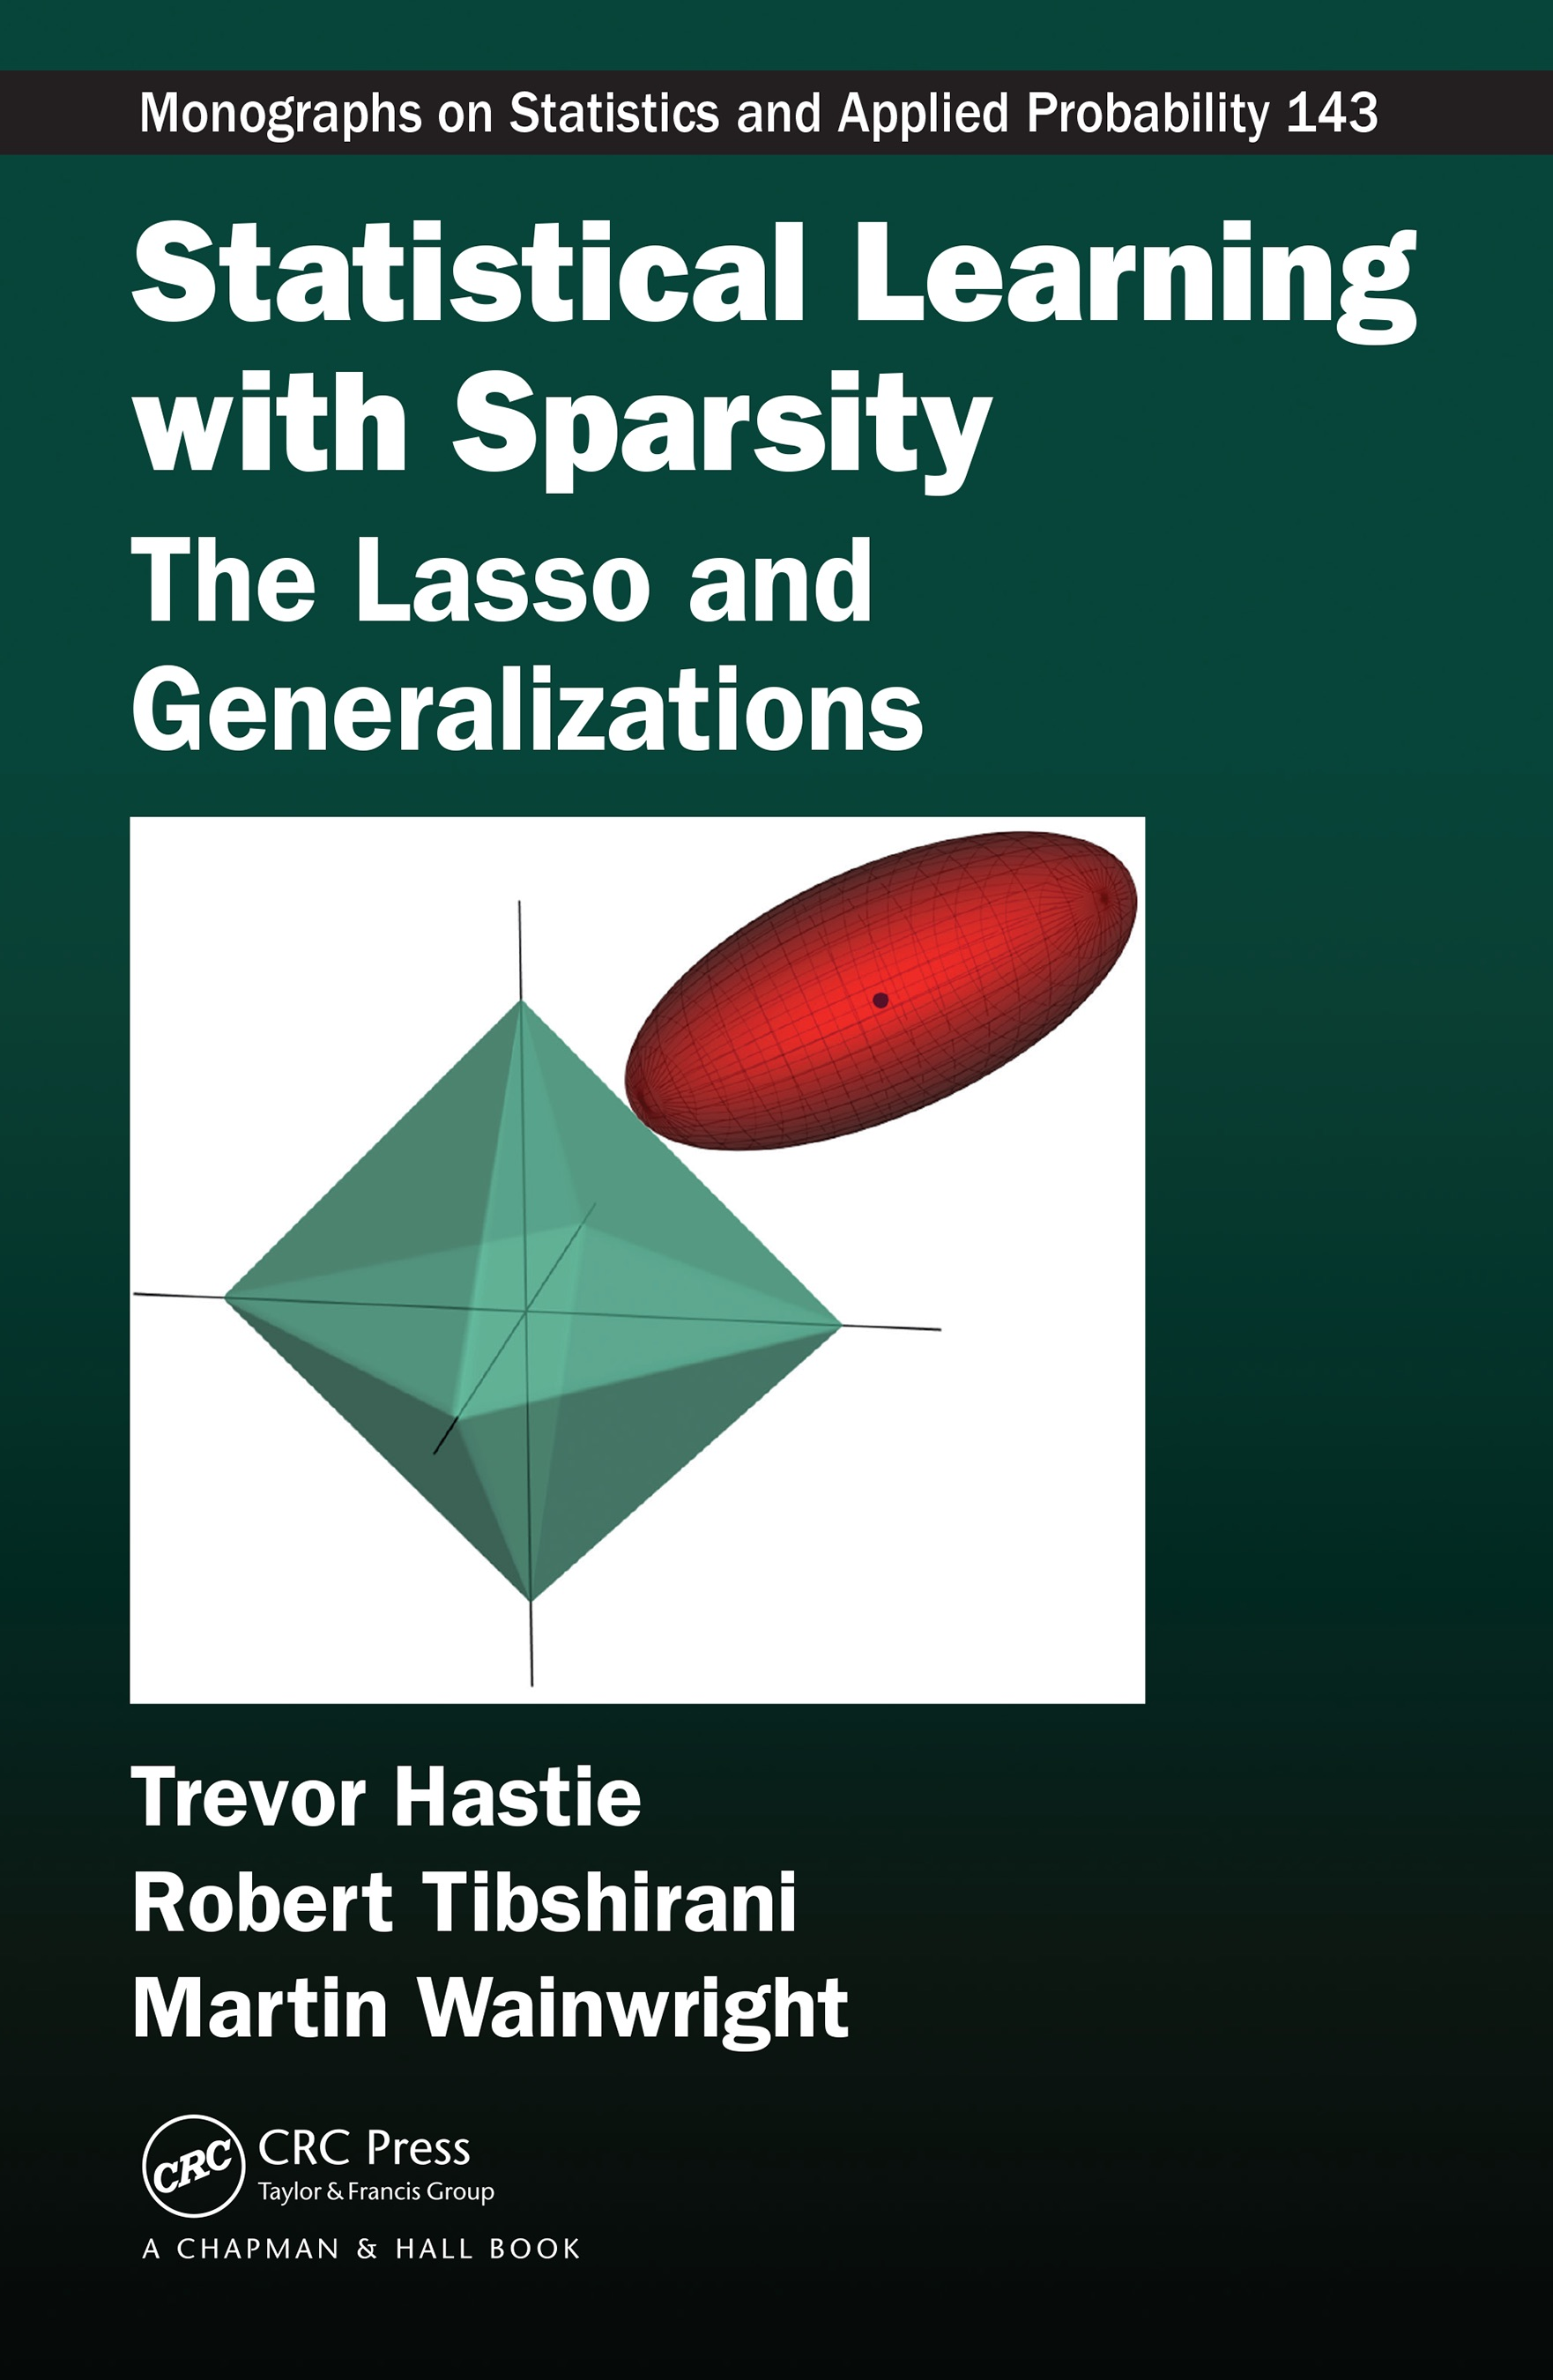
\includegraphics[scale = 0.05]{sls.jpg}
\end{center}
\begin{itemize}
\item Suppose that $Y \approx f(X) + \epsilon$, where $f$ depends \emph{sparsely} on $X$.
\item Can we exploit the sparsity to obtain an estimate of $I(X; Y)$?
\end{itemize}
\end{frame}


\begin{frame}
\frametitle{Our proposal}
Suppose we observe pairs $(X_i,Y_i)_{i=1}^n$ iid from density $p(x, y)$.
\begin{enumerate}
\item Estimate a (sparse) regression model for $\E[y|x]$.
\item Estimate the noise model for $Y$.
\item Estimate the \emph{identification risk} $p$ using cross-validation.
\item Use the identification risk to obtain a lower bound for the mutual information $I(X; Y)$:
\[
I(X; Y) \geq f(p)
\]
where $f$ is a function that we derive theoretically. 
\end{enumerate}
\end{frame}

\begin{frame}
\frametitle{Multiple-response regression}
\begin{itemize}
\item Pairs $(x_i,y_i)_{i=1}^n$, where $X$ is $p$-dimensional and $Y$ is $q$-dimensional.
\item Data matrices $\bX_{n \times p}$, $\bY_{n \times q}$.
\item For each column of $Y$, fit sparse model $Y^{(i)} \approx X^T \beta^{(i)}  + \epsilon$, e.g. by using elastic net (Zou 1998), 
\[
\hat{\beta}^{(i)} = \text{argmin}_\beta ||\bX^T \beta^{(i)} - Y^{(i)}||^2 + \lambda_2 ||\beta^{(i)}||_2^2 + \lambda_1 ||\beta^{(i)}||_1
\]
\item Or, fit a \emph{random forest} model for each column of $Y$ (Breiman 2001)
\end{itemize}
\end{frame}


\begin{frame}
\frametitle{Regression vs Identification loss}
\begin{itemize}
\item Independent \emph{test set} $(x_i^*, y_i^*)_{i=1}^k$. 
\item Use model to predict $\hat{y}_i^* = (x_i^*)^T \hat{B}$ for $i = 1,\hdots, k$.
\end{itemize}
Two ways to evaluate the predictive accuracy of the regression model:
\begin{itemize}
\item Regression (mean squared-error) loss:
\[
\text{MSE} = \frac{1}{k} \sum_{i=1}^k ||y_i^* - \hat{y}_i^*||^2.
\]
\item Identification loss:
\[
\text{IdLoss}_k = \frac{1}{k} \sum_{i=1}^k (1 - I\{\hat{y}_i^* \text{ is nearest neighbor of }y_i^*\}).
\]
\end{itemize}
\end{frame}

\begin{frame}
\frametitle{Cross-validated loss}
Leave-$k$-out cross-validation (L$k$oCV) can be used for both squared-error loss and identification loss.
\begin{itemize}
\item Start with a dataset $(x_i,y_i)_{i=1}^N$.
\item Let $n = N-k$.  Consider all ${N}\choose{k}$ partitions of the dataset into a test set $(\bX, \bY)$ and training set $(\bX^*, \bY^*)$.
\item For each partition, compute the loss.
\item Define the L$k$oCV loss as the average loss over ${N}\choose{k}$ partitions.
\end{itemize}
\emph{Computational note}.  One can subsample to avoid computing all
${N}\choose{k}$ partitions.  In particular, if $m = N/k$, then one can
use $m$-fold cross-validation which uses $m$ partitions that have
disjoint test sets.
\end{frame}

\begin{frame}
\frametitle{Identification loss and mutual information}
\begin{itemize}
\item Define the identification risk as the expected identification loss
\[
\text{IdRisk}_k = \E[\text{IdLoss}_k]
\]
\item Define the Bayes risk as the identification risk given the \emph{true} model parameters.
Hence,
\[
\text{BayesRisk}_k \leq \text{IdRisk}_k.
\]
%\item \textbf{High-dimensional result.}  In a certain high-dimensional
%  asymptotic regime, there exists a limiting functional relationship
%\[
%\text{Bayes risk} = \pi_k(\sqrt{2 I(X; Y)})
%\]
\item \textbf{Theorem.} (Z., Benjamini 2016) There exists a function $g_k$ such that
%For every $k \geq 2$, there exists a function $g_k$ such that
\[I(X; Y) \geq g_k(\text{IdRisk}_k).\]
%$\Box$.
\item Resulting estimator:
\[
\hat{I}_{IdLoss}(X; Y) = g_k(\text{IdLoss}_k)).
\]
%\item \emph{Remark.} Although $\text{IdLoss}_k$ is unbiased for $\text{IdRisk}_k$, $g_k$ is nonlinear so $\hat{I}_{IdLoss}$ may be biased.
\end{itemize}
\end{frame}

\begin{frame}
\frametitle{Functions}

Illustration of $C_k = g_k^{-1}$
\begin{center}
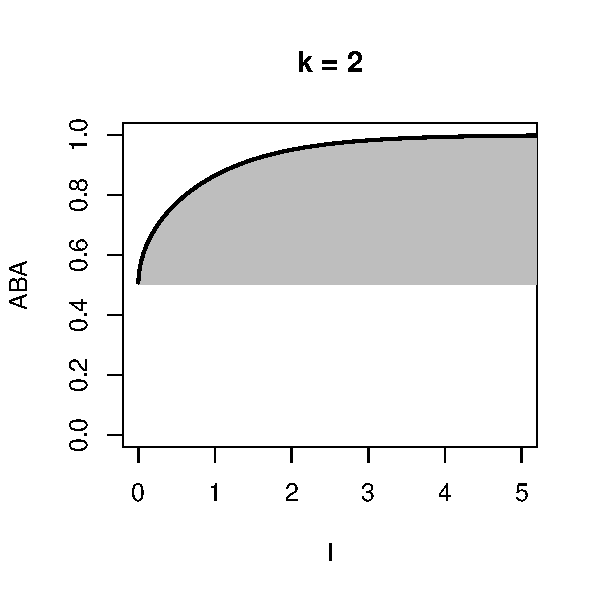
\includegraphics[scale = 0.34]{ck_2.pdf}
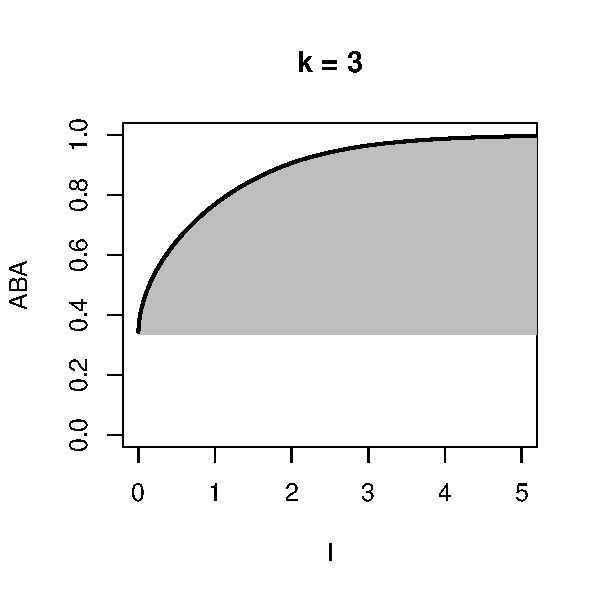
\includegraphics[scale = 0.34]{ck_3.pdf}
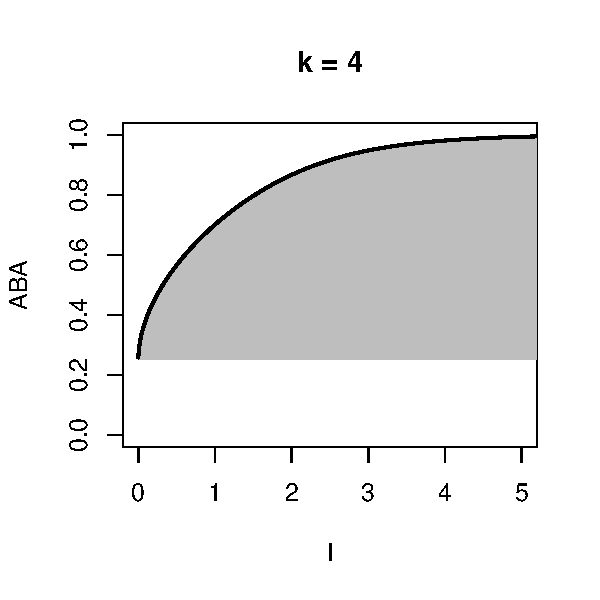
\includegraphics[scale = 0.34]{ck_4.pdf}
\end{center}
As information increases, the maximal identification risk goes to 0.
[note: pictures need to be rotated]
%We find these curves using \emph{variational calculus}.

\end{frame}

\begin{frame}
\frametitle{Simulation}


\begin{center}
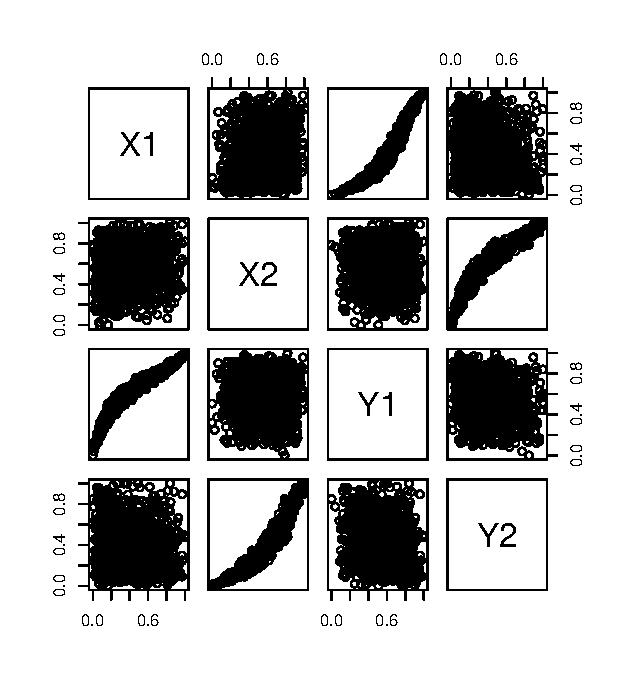
\includegraphics[scale = 0.34]{../idloss/sim1_pairs.pdf}
\end{center}
\begin{itemize}
\item Generate data: $(Y_1, Y_2) = f(X_1, X_2, \epsilon)$ where $f$ is nonlinear.
\item $n = 1000$.
\item Compare Nearest-Neighbor estimator (Mnatsakov et al, 2008, implemented in {\tt FNN}) with our method using \emph{Random Forest}.
\item Add extra noise dimensions $X_3, X_4, \hdots$.
\end{itemize}

%We find these curves using \emph{variational calculus}.

\end{frame}

\begin{frame}
\frametitle{Simulation Results}

True $I(X; Y) = 4.615$.

\begin{center}
\begin{tabular}{c||c|c|c}
Extra dim & NN & RF $k = 10$ & RF $k=20$\\
0 & \textbf{4.445} & 3.989 & 3.924\\
1 & 3.040 & \textbf{3.645} & 3.610\\
2 & 1.773 & \textbf{3.249} & 3.182
\end{tabular}
\end{center}

%We find these curves using \emph{variational calculus}.

\end{frame}

\begin{frame}
\frametitle{Application to gene expression time series}
to be contd
\end{frame}

\end{document}

\begin{frame}
\frametitle{Gaussian example}
To help think about these problems, consider a concrete example:
\begin{itemize}
\item Let $\bX \sim N(0, I_d)$ and 
$\bY|\bX \sim N(\bX,\sigma^2 I_d)$.
\item We draw stimuli $\bx^{(1)}, \hdots, \bx^{(K)} \sim N(0, I_d)$ i.i.d.
\item For each stimulus $\bx^{(i)}$, we draw observations $\by^{(i, j)} = \bx^{(i)} + \epsilon^{(i, j)}$, where $\epsilon^{(i, j)} \sim N(0, \sigma^2 I_d)$.
\end{itemize}
\begin{center}
\begin{tabular}{ccc}
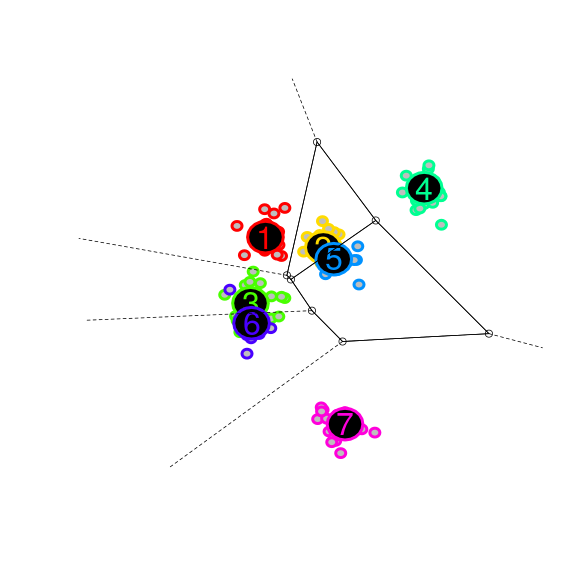
\includegraphics[scale = 0.2, clip = true, trim = 0.6in 0.2in 0.6in 0.2in]{../info_theory_paper/gaussian_figure1a.png} &
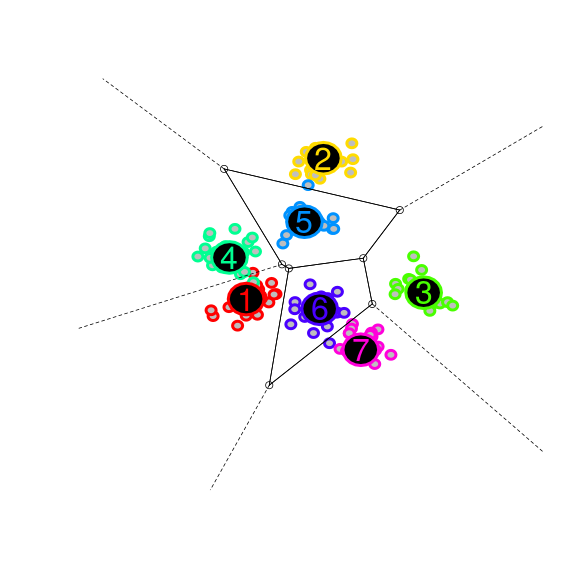
\includegraphics[scale = 0.2, clip = true, trim = 0.6in 0.2in 0.6in 0.2in]{../info_theory_paper/gaussian_figure1b.png} &
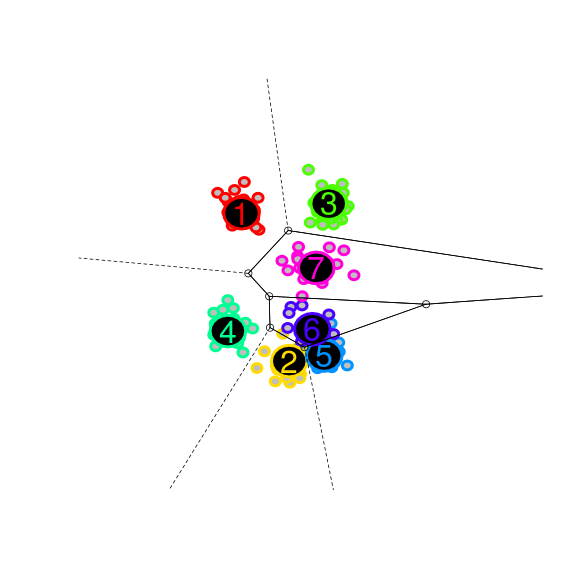
\includegraphics[scale = 0.2, clip = true, trim = 0.6in 0.2in 0.6in 0.2in]{../info_theory_paper/gaussian_figure1c.png}
\end{tabular}
\end{center}
\end{frame}

\begin{frame}
\frametitle{Gaussian example}
The mutual information is given by
\[
I(\bX;\bY) = \frac{d}{2}\log(1 + \frac{1}{\sigma^2}).
\]

Define
\[
Z_i = -\frac{1}{2\sigma^2}||Y^* - X_i||^2.
\]
The Bayes risk can be written
\[
\text{BayesRisk} = \Pr[Z_* < \max_{i=1}^{K-1} Z_i].
\]
\end{frame}

\begin{frame}
\frametitle{Gaussian example: Bayes risk}
\begin{itemize}
\item To make the problem even easier, we use another time-honored technique: the central limit theorem.
\item Letting $d \to \infty$, the scores
\[
Z_i = -\frac{1}{2\sigma^2} ||\bY - \bx||^2 = -\frac{1}{2\sigma^2} \sum_{i=1}^d ||Y_i - x_i||^2
\]
have a jointly multivariate distribution in the limit:
\end{itemize}
\[
\begin{bmatrix}
Z_*\\
Z_1\\
\vdots\\
Z_{K-1}
\end{bmatrix} \stackrel{d}{\to} N\left(
\begin{bmatrix}
-\frac{d}{2}\\
-\frac{d}{2} - \frac{d}{\sigma^2}\\
\vdots\\
-\frac{d}{2} - \frac{d}{\sigma^2}
\end{bmatrix},
\begin{bmatrix}
\frac{d}{2} & \frac{d}{2} & \cdots & \frac{d}{2}\\
\frac{d}{2} & \frac{d}{2} + \frac{2d}{\sigma^2} & \cdots & \frac{d}{2} + \frac{d}{\sigma^2}\\
\vdots & \vdots & \ddots & \vdots\\
\frac{d}{2} & \frac{d}{2} + \frac{d}{\sigma^2} & \cdots & \frac{d}{2} + \frac{2d}{\sigma^2}
\end{bmatrix}
\right).
\]
\end{frame}

\begin{frame}
\frametitle{Gaussian example: Bayes risk}

Assume $(Z_*, Z_1,\hdots, Z_{K-1})$ have a normal distribution with the given moments.

We can compute
\[
\text{BayesRisk}_k = \Pr[Z_* < \max_{i=1}^{K-1} Z_i]
\]
by writing
\[
Z_i = \frac{\Cov(Z_*, Z_i)}{\Var(Z_*)} (Z_* - \E Z_*) + \sqrt{\Var(Z_i) - \frac{\Cov(Z_*, Z_i)^2}{\Var(Z_*)}} W_i,
\]
where $W_i$ are i.i.d. standard normal.

This yields
\[
\Pr[Z_* < \max_{i=1}^{K-1} Z_i] = \Pr[N(\mu, \nu^2) < \max_{i=1}^{K-1} W_i]
\]
where
\[
\mu = \frac{\E[Z_* - Z_i]}{\sqrt{\frac{1}{2}\Var(Z_i - Z_j)}},\ \nu^2 = \frac{\Cov(Z_* - Z_i, Z_* - Z_j)}{\frac{1}{2}\Var(Z_i - Z_j)}
\]
for $i \neq j \neq K$.

\end{frame}

\begin{frame}
\frametitle{Gaussian example: Bayes risk}
Finally, we get
\[
\text{BayesRisk} = \Pr[Z_* < \max_{i=1}^{K-1} Z_i] \to \pi_K\left(\frac{\sqrt{d}}{\sigma}\right)
\]
where
\[
\pi_K(\mu) =  1 - \int_{-\infty}^\infty \phi(z-\mu) (1-\Phi(z))^{K-1} dz.
\]
\end{frame}

\begin{frame}
\frametitle{Sidenote: interpretation of $\pi_K$}

The function $\pi_K(\mu)$ gives the probability that a $N(\mu, 1)$
variable is smaller than the minimum of $K-1$ other $N(0, 1)$ variables
(all independent.)

Hence $\pi_K(0) = \frac{K-1}{K}$ due to symmetry.  (This is also the misclassification rate from pure guessing.)

\begin{center}

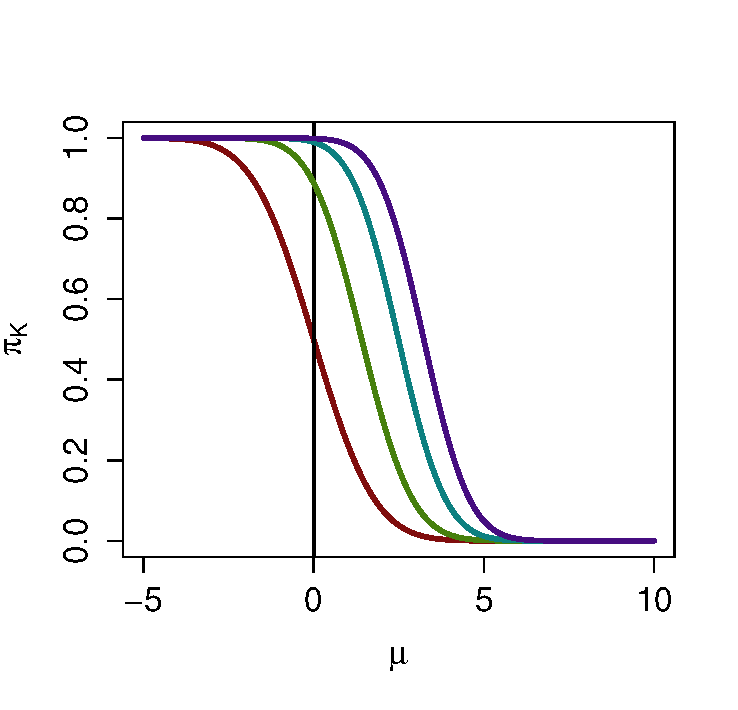
\includegraphics[scale = 0.5, clip=true, trim=0 0.2in 0 0.5in]{../info_theory_sims/illus_piK.pdf}

Legend: $K = \{$
\sethlcolor{color1}
\textbf{\textcolor{white}{\SoulColor\hl{ 2 }}}, 
\sethlcolor{color2}
\textbf{\textcolor{white}{\SoulColor\hl{ 9 }}},
\sethlcolor{color3}
\textbf{\textcolor{white}{\SoulColor\hl{ 99 }}},
\sethlcolor{color4}
\textbf{\textcolor{white}{\SoulColor\hl{ 999 }}}$\ \}$
\end{center}

\end{frame}


\begin{frame}
\frametitle{Gaussian example: Bayes risk}

Recall that
\[
I(\bX; \bY) =  \frac{d}{2}\log(1 + \frac{1}{\sigma^2}),
\]
while
\[
\text{BayesRisk}_k = \pi_K(\sqrt{d}/\sigma).
\]

Hence Bayes risk is \emph{not} a function of $I(\bX; \bY)$!
\end{frame}


\begin{frame}
\frametitle{Gaussian example: Low SNR limit}
However, what if we consider a limit where the noise level $\sigma^2$ increases with $d$?

Fix some $\sigma^2_1 > 0$, and let $\sigma^2_d  = d \sigma^2_1$.

Then when $d$ is large,
\[
I(\bX; \bY) = \frac{d}{2}\log(1 + \frac{1}{d \sigma^2_1}) \approx \frac{d}{2}\frac{1}{d\sigma^1} = \frac{1}{2\sigma^2_1}.
\]

We get
\[
\text{Bayes risk} = \pi_k(\sqrt{2 I(\bX; \bY)})
\]
in the limit!
\end{frame}

\begin{frame}
\frametitle{Low SNR limit: generalization}

In a sequence of gaussian models of increasing dimensionality with
\[
\lim_{d \to \infty} I(\bX; \bY) \to \iota < 0,
\]
we get an exact relationship between the limiting mutual information and the average Bayes error,
\[
\text{BayesRisk}_k = \pi_K(\sqrt{2\iota}).
\]

\textbf{This limiting relationship holds more generally!}
\end{frame}

\begin{frame}
\frametitle{Low SNR theorem}

\textbf{Theorem. }\emph{
Given an exponential family sequence model $p_d(\bx, \by)$,
for random variates $(\bX^{[d]}, \bY^{[d]}) \sim p_d(\bX, \bY)$, we have
\[
\lim_{d \to \infty} I(\bX^{[d]}, \bY^{[d]})  = \iota < \infty
\]
for some constant $\iota < \infty$;
and the limiting $K$-class average Bayes error is given by
\[
\lim_{d \to \infty} \text{ABE} = \pi_K(\sqrt{2\iota}).
\]
}

\note{
The proof is basically an application of first order Taylor expansion, using the fact that for small $\theta$,
\[
b_\theta(x, y) \approx b_X(x) b_Y(y) \exp[\theta u(x, y)] \approx b_X(x) b_Y(y) (1 + \theta u(x, y)),
\]
allowing us to relate moments of the joint distribution of $p(\bx,
\by)$ (which give the mutual information) with moments of the
product-marginal $p(\bx)p(\by)$ (which give the ABE).
}
\end{frame}

\begin{frame}
\frametitle{The low-SNR estimator of $I(\bX;\bY)$}

We are willing to bet that the relationship 
\[\text{ABE} \approx \pi_K(\sqrt{2\iota})\]
holds in much greater generality than we managed to prove--namely,
whenever $I(\bX; \bY) \ll p$, and the scores $Z_i$ are approximately
jointly multivariate normal.\newline

Based on these assumptions, our proposed estimator for mutual information is
\[
\hat{I}_{ls}(\bX; \bY) = \frac{1}{2}\pi_K^{-1}(\widehat{\text{ABE}})^2
\]
where $\widehat{\text{ABE}}$ is the test error of the classifier.
(The subscript $ls$ stands for low-SNR.)
\end{frame}

\section{Results}

\begin{frame}
\frametitle{Simulation study}
\emph{Models.}
\begin{itemize}
\item Multiple-response logistic regression model
\[
X \sim N(0, I_p)
\]
\[
Y \in \{0,1\}^q
\]
\[
Y_i|X = x \sim \text{Bernoulli}(x^T B_i)
\]
where $B$ is a $p \times q$ matrix.
\end{itemize}

\emph{Methods.}
\begin{itemize}
\item \text{Nonparametric}: $\hat{I}_0$ naive estimator, $\hat{I}_\alpha$ anthropic correction.
\item \text{ML-based}: $\hat{I}_{CM}$ confusion matrix, $\hat{I}_F$ Fano, $\hat{I}_{LS}$ low-SNR method.
\end{itemize}
\end{frame}

\begin{frame}
\frametitle{Fig 1. Low-dimensional results ($q = 3$)}
Sampling distribution of $\hat{I}$ for \small{$\{p = 3$, $B = \frac{4}{\sqrt{3}} I_3$, $K = 20$, $r = 40\}$.}

True parameter $I(X; Y) = 0.800$ \emph{(dotted line.)}
\begin{center}
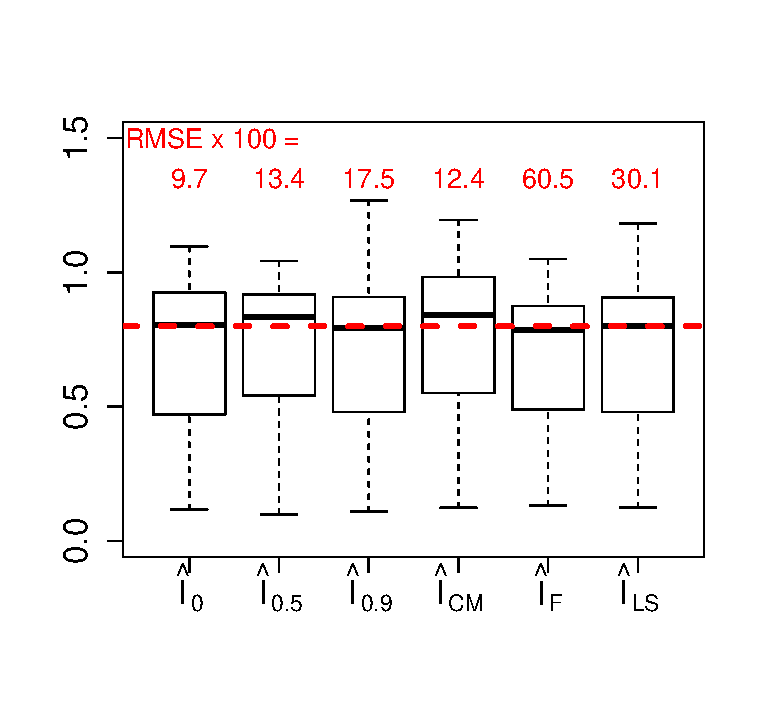
\includegraphics[scale = 0.5, clip = true, trim = 0 0.5in 0 0.5in]{../info_theory_sims/fig1.pdf}
\end{center}
Na\"{i}ve estimator performs best!  $\hat{I}_{LS}$ not effective.
\end{frame}

\begin{frame}
\frametitle{Fig 2. High-dimensional results ($q = 50$)}
Sampling distribution of $\hat{I}$ for \small{$\{p = 50$, $B = \frac{4}{\sqrt{50}} I_{50}$, $K = 20$, $r = 8000\}$.}

True parameter $I(X; Y) = 1.794$ \emph{(dashed line.)}
\begin{center}
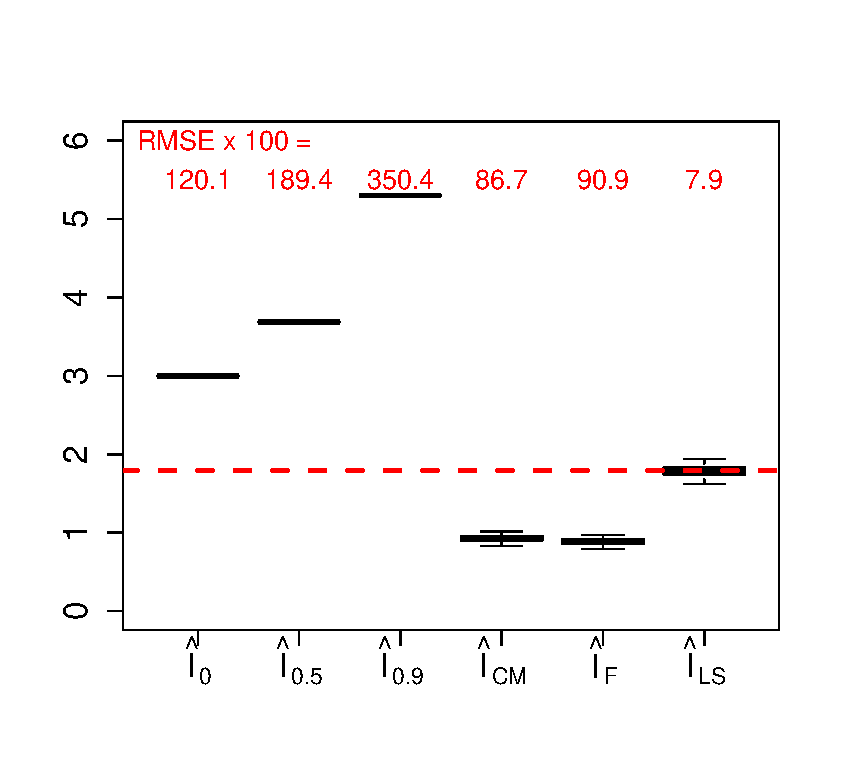
\includegraphics[scale = 0.5, clip = true, trim = 0 0.5in 0 0.5in]{../info_theory_sims/fig2.pdf}
\end{center}
Non-parametric methods extremely biased.
\end{frame}

\begin{frame}
\frametitle{Fig 3. Dependence on $n$ ($q = 10$)}
Estimation path of $\hat{I}_{LS}$ and $\hat{I}_\alpha$ as $n$ ranges from $10$ to $8000$.

\small{$\{p = 10$, $B = \frac{4}{\sqrt{10}} I_{10}$, $K = 20\}$.
True parameter $I(X; Y) = 1.322$ \emph{(dashed line.)}}

\begin{center}
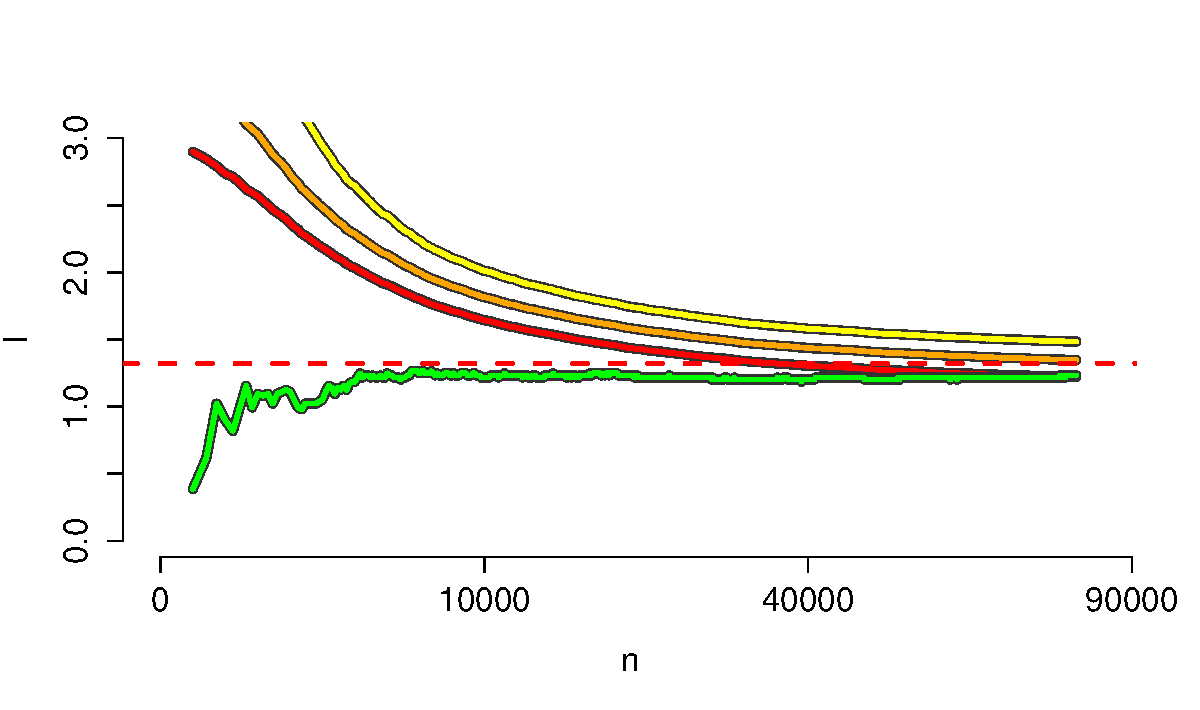
\includegraphics[scale = 0.4]{../info_theory_sims/fig3.pdf}
\end{center}

Legend: \textbf{\textcolor{green}{\SoulColor\hl{ -- }}} = $\hat{I}_{LS}$, \textcolor{red}{\SoulColor\hl{ -- }} = $\hat{I}_0$, \textcolor{orange}{\SoulColor\hl{ -- }} = $\hat{I}_{0.5}$,
\textbf{\textcolor{yellow}{\SoulColor\hl{ -- }}} = $\hat{I}_{0.9}$.

\end{frame}

\begin{frame}
\frametitle{Fig 4. Dependence on true $I(X; Y)$ ($q = 10$)}

\small{$\{p = 10$, $B = [0, 200]\times \frac{1}{\sqrt{10}}I_{10}$, $r = 1000$, $K = 20\}$.}

\begin{center}
\textbf{Estimated $\hat{I}$ vs true $I$.} 

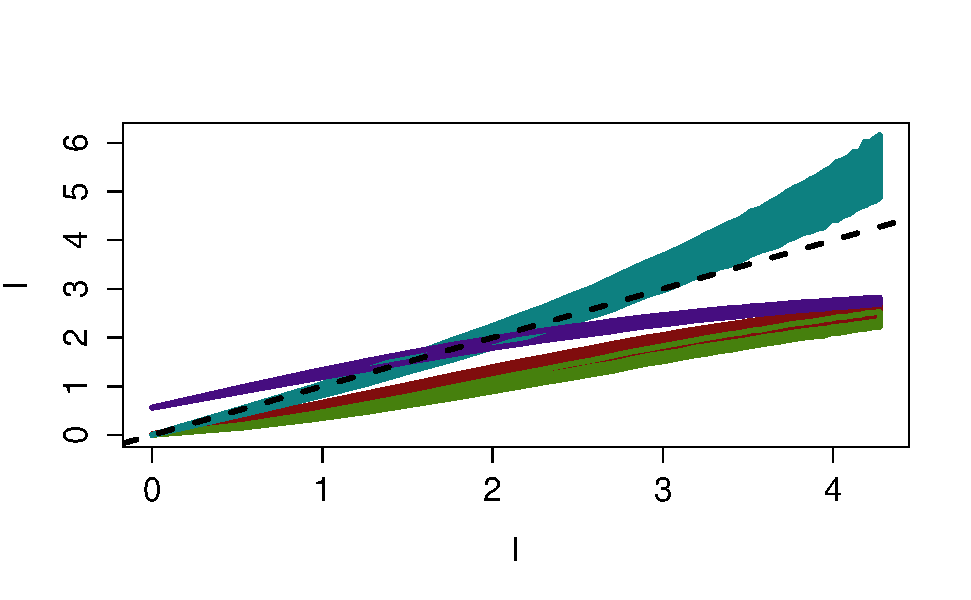
\includegraphics[scale = 0.5, clip=true, trim=0.4in 0.5in 0 0.5in]{../info_theory_sims/fig4.pdf}

Bands depict 80\% central percentiles.

Legend: 
\sethlcolor{color3}
\textbf{\textcolor{color3}{\SoulColor\hl{ -- }}} = $\hat{I}_{LS}$, 
\sethlcolor{color4}
\textcolor{color4}{\SoulColor\hl{ -- }} = $\hat{I}_0$,
\sethlcolor{color1}
\textcolor{color1}{\SoulColor\hl{ -- }} = $\hat{I}_{CM}$,
\sethlcolor{color2}
\textbf{\textcolor{color2}{\SoulColor\hl{ -- }}} = $\hat{I}_{F}$.

\end{center}

\end{frame}


\begin{frame}
\frametitle{Fig 5. Dependence on $K$ given fixed $N$ ($q = 10$)}
Sampling distribution of $\hat{I}_{LS}$ for \small{$\{p = 10$, $B = \frac{4}{\sqrt{10}} I_{10}$, $N = 80000\}$,

and $K = \{5, 10, 15, 20, \hdots, 80\}$, $r = N/k$.}

True parameter $I(X; Y) = 1.322$ \emph{(dashed line.)}
\begin{center}
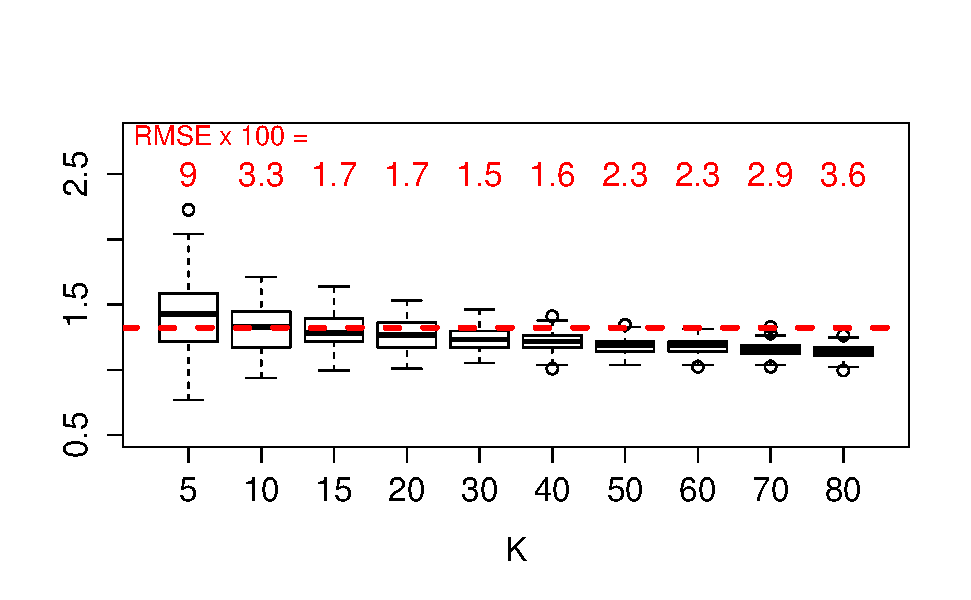
\includegraphics[scale = 0.6, clip = true, trim = 0 0.5in 0 0.5in]{../info_theory_sims/fig5a.pdf}
\end{center}

Decreasing variance as $K$ increases. Bias at large and small $K$.
\end{frame}

\begin{frame}
\frametitle{Fig 6. Non-identity $B$ ($q = 40$)}

$p = 20$ and $q = 40$, entries of $B$ are iid $N(0, 0.025)$.

$K=20$, $r = 8000$, true $I(X; Y) = 1.86$ \emph{(dashed line.)}

\begin{center}
\textbf{Sampling distribution of $\hat{I}$.}
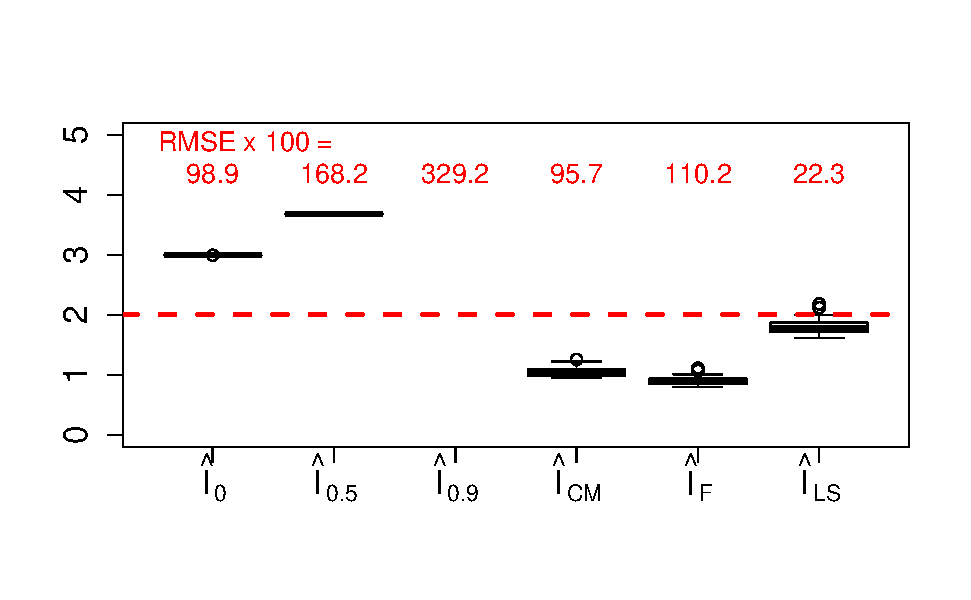
\includegraphics[scale = 0.6, clip = true, trim = 0 0.5in 0 0.5in]{../info_theory_sims/fig6.pdf}
\end{center}


\end{frame}

\begin{frame}
\frametitle{Conclusions}
\begin{itemize}
\item We derive a relationship between average Bayes error (ABE) and mutual
  information (MI), motivating a novel estimator $\hat{I}_{LS}$.
\item Theory based on high dimensional, low SNR limit,
where \[\text{ABE} \leftrightarrow \text{MI}.\]
\item In ideal settings for supervised learning, ABE can be estimated
  effectively and $\hat{I}_{LS}$ can recover MI at much lower sample
  sizes than nonparametric methods.
\item In simulations, $\hat{I}_{LS}$ works better than Fano's
  inequality or the confusion matrix approach.
\end{itemize}
\end{frame}

\begin{frame}
\frametitle{References}
\begin{itemize}
\item Cover and Thomas.  Elements of information theory.
\item Muirhead.  Aspects of multivariate statistical theory.
\item van der Vaart.  Asymptotic statistics.
\end{itemize}
\end{frame}

\end{document}




\begin{itemize}
\item 
\item Define a distribution $p(\bx)$ supported on $\mathcal{X}$.  \emph{In practice, $p(\bx)$ may be represented as a large image database.}
\item Sample stimuli $\bX^{(1)}, \hdots, \bX^{(K)}$ from $p(x)$. \emph{I.e., draw $K$ images from the image database.}
\item For $i = 1,\hdots, K$, present the subject with stimulus
  $\bX^{(1)}$, record the neural response $\bY^{(i, j)}$.  For each
  stimulus, obtain repeats $j = 1,\hdots, r$.
\end{itemize}








